\documentclass[12pt,a4paper]{report}

\usepackage{cmap}
\usepackage[T1]{fontenc}
\usepackage{lmodern}
\usepackage[utf8]{inputenc} % pentru suport diacritice
\usepackage[romanian]{babel} % setări pentru limba română 
\renewcommand\familydefault{\sfdefault} % sans serif

\usepackage[margin=2.54cm]{geometry}	% dimensiuni pagină și margini
\usepackage{graphicx} % support the \includegraphics command and options

% formatting sections and subsections
\usepackage{textcase}
\usepackage[titletoc, title]{appendix}
\usepackage{titlesec}
\titleformat{\chapter}{\large\bfseries\MakeUppercase}{\thechapter}{2ex}{}
\titlespacing*{\chapter}{0pt}{-29.5pt}{20pt}
\titleformat*{\section}{\large\bfseries}
\titleformat*{\subsection}{\large\bfseries}
\titleformat*{\subsubsection}{\normalsize}

\usepackage{chngcntr}
\counterwithout{figure}{chapter} % no chapter number in figure labels
\counterwithout{table}{chapter} % no chapter number in table labels
\counterwithout{equation}{chapter} % no chapter number in equation labels

\usepackage{booktabs} % for much better looking tables
\usepackage[section]{placeins} % don't let tables/figures float past a \section boundary
\usepackage{url} % Useful for inserting web links nicely
\usepackage[bookmarks,unicode,hidelinks]{hyperref}

\usepackage{array} % for better arrays (eg matrices) in maths
\usepackage{paralist} % very flexible & customisable lists (eg. enumerate/itemize, etc.)
\usepackage{verbatim} % adds environment for commenting out blocks of text & for better verbatim
\usepackage{subfig} % make it possible to include more than one captioned figure/table in a single float
\usepackage{enumitem}
\setlist{noitemsep}

%%% HEADERS & FOOTERS
\usepackage{fancyhdr}
\pagestyle{empty}
\renewcommand{\headrulewidth}{0pt}
\renewcommand{\footrulewidth}{0pt}
\lhead{}\chead{}\rhead{}
\lfoot{}\cfoot{\thepage}\rfoot{}



\newcommand{\HeaderLineSpace}{0.1cm}
\newcommand{\UniTextRO}{UNIVERSITATEA NAȚIONALĂ DE ȘTIINȚĂ ȘI TEHNOLOGIE POLITEHNICA DIN BUCUREȘTI \\[\HeaderLineSpace] 
FACULTATEA DE AUTOMATICĂ ȘI CALCULATOARE \\[\HeaderLineSpace]
DEPARTAMENTUL DE CALCULATOARE\\}
\newcommand{\DiplomaRO}{PROIECT DE DIPLOMĂ}
\newcommand{\AdvisorRO}{Coordonator științific:}
\newcommand{\BucRO}{BUCUREȘTI}

\newcommand{\UniTextEN}{NATIONAL UNIVERSITY OF SCIENCE AND TECHNOLOGY POLITEHNICA OF BUCHAREST \\[\HeaderLineSpace]
FACULTY OF AUTOMATIC CONTROL AND COMPUTERS \\[\HeaderLineSpace]
COMPUTER SCIENCE AND ENGINEERING DEPARTMENT\\}
\newcommand{\DiplomaEN}{DIPLOMA PROJECT}
\newcommand{\AdvisorEN}{Thesis advisor:}
\newcommand{\BucEN}{BUCHAREST}

\newcommand{\frontPage}[6]{
\begin{titlepage}
\begin{center}
{\Large #1}  % header (university, faculty, department)
\vspace{50pt}
\begin{tabular}{p{6cm}p{4cm}}

\includegraphics[scale=0.8]{pics/upb-logo.jpg} &
	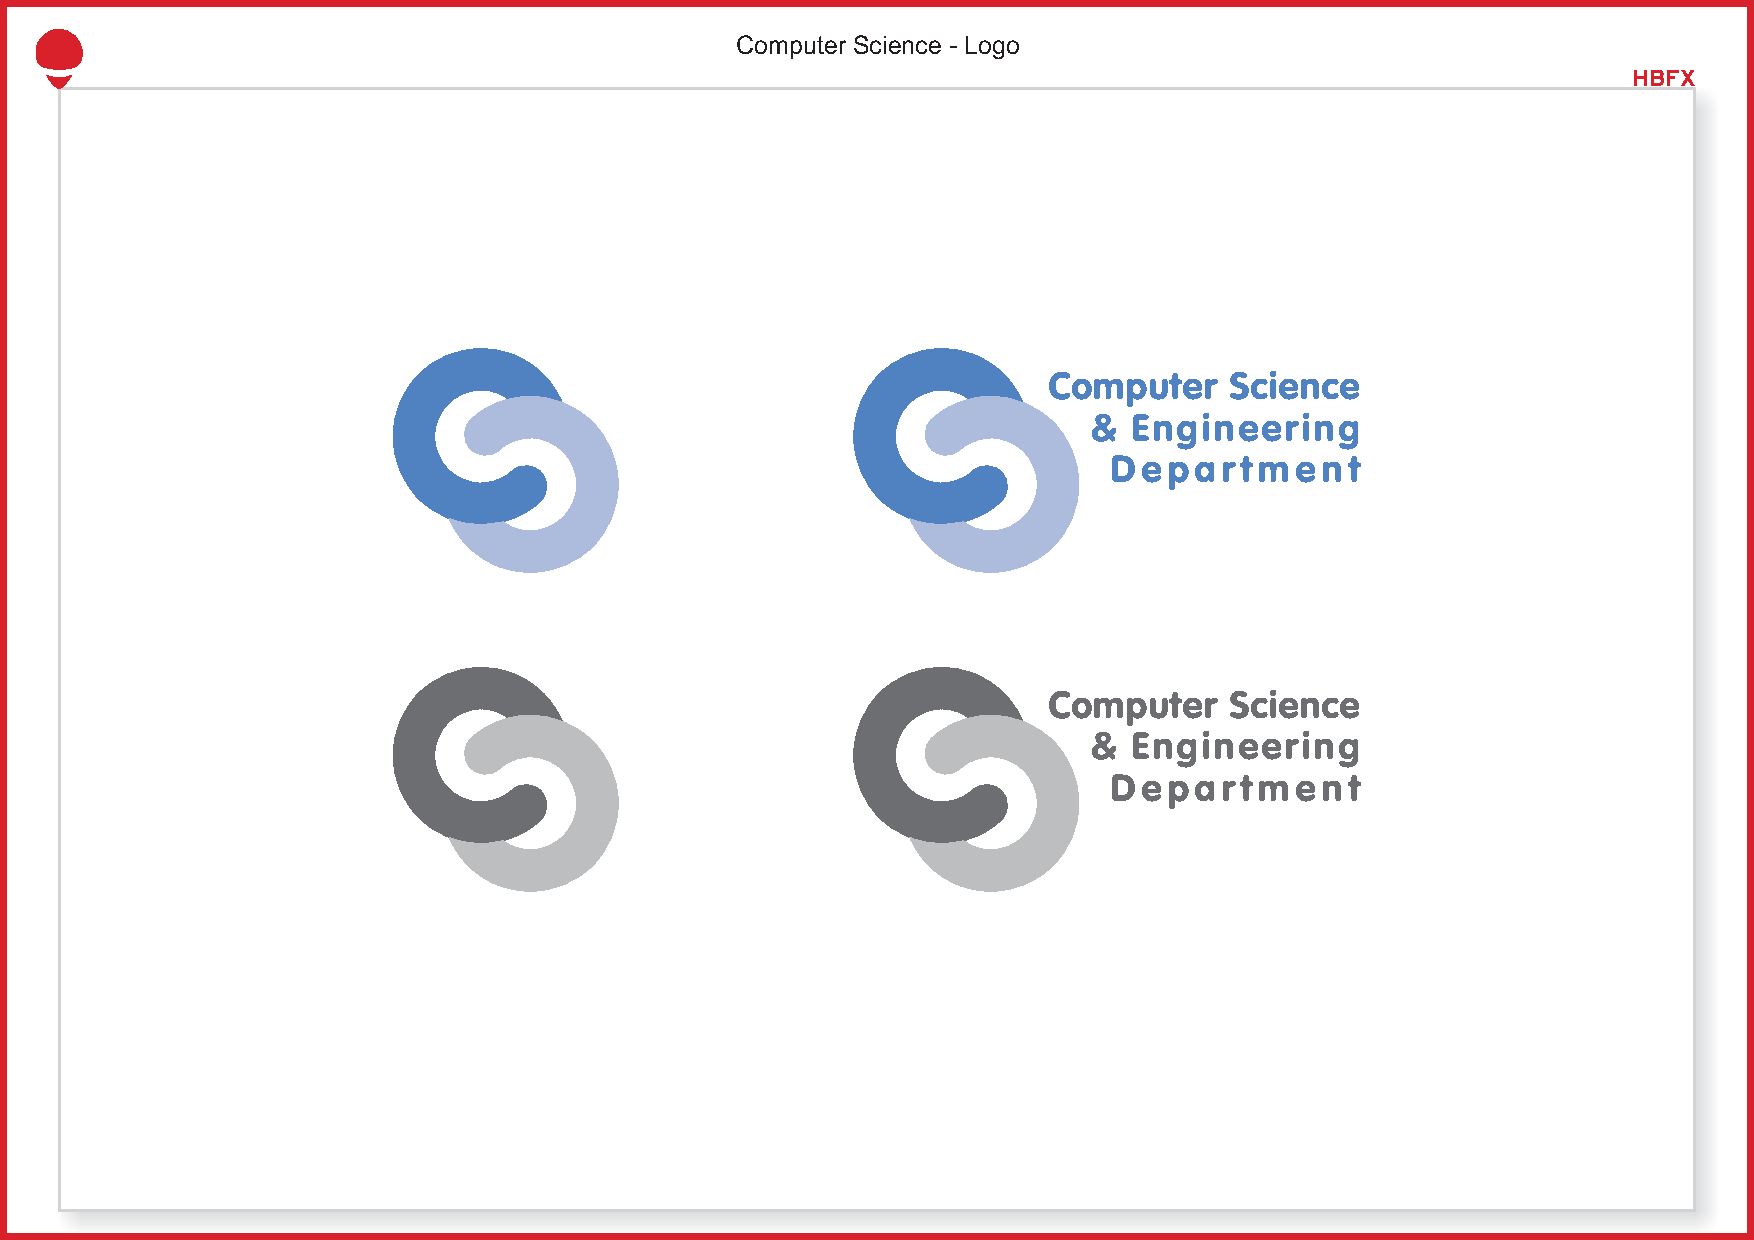
\includegraphics[scale=0.5,trim={14cm 11cm 2cm 5cm},clip=true]{pics/cs-logo.pdf}
\end{tabular}

\vspace{105pt}
{\Huge #2}\\                           % diploma project text
\vspace{40pt}
{\Large #3}\\ \vspace{0pt}  % project title
% {\Large #4}\\                          % project subtitle
\vspace{40pt}
{\LARGE \Name}\\                   % student name
\end{center}
\vspace{60pt}
\begin{tabular*}{\textwidth}{@{\extracolsep{\fill}}p{6cm}r}
&{\large\textbf{#5}}\vspace{10pt}\\      % scientific advisor
&{\large \Advisor}                                    % advisor name
\end{tabular*}
\vspace{20pt}
\begin{center}
{\large\textbf{#6}}\\                                % bucharest
\vspace{0pt}
{\normalsize \Year}
\end{center}
\end{titlepage}
}

\newcommand{\frontPageRO}{\frontPage{\UniTextRO}{\DiplomaRO}{\ProjectTitleRO}{\ProjectSubtitleRO}{\AdvisorRO}{\BucRO}}
\newcommand{\frontPageEN}{\frontPage{\UniTextEN}{\DiplomaEN}{\ProjectTitleEN}{\ProjectSubtitleEN}{\AdvisorEN}{\BucEN}}

\linespread{1.2}
\setlength\parindent{0pt}
\setlength\parskip{.28cm}
\raggedbottom

%% Abstract macro
\newcommand{\AbstractPage}{
\begin{titlepage}
\textbf{\large SINOPSIS}\par
\AbstractRO\par\vfill
\textbf{\large ABSTRACT}\par
\AbstractEN \vfill
\end{titlepage}
}

%% Thank you macro
\newcommand{\ThanksPage}{
\begin{titlepage}
{\noindent \large\textbf{MULȚUMIRI}}\\
\Thanks
\end{titlepage}
}



%%%%%%%%%%%%%%%%%%%%%%%%%%%%%%%%%%%%%%%%%%%%%%%%%%   
%%
%%          End of template definitions
%%   
%%%%%%%%%%%%%%%%%%%%%%%%%%%%%%%%%%%%%%%%%%%%%%%%%%


%%% Puteți elimina aceste linii din lucrare, servesc numai pentru template.
\newcommand{\worktype}[1]{[\textit{#1}] }
\newcommand{\dezvoltare}{\worktype{Dezvoltare de produs}}
\newcommand{\cercetare}{\worktype{Cercetare}}
\newcommand{\ambele}{\worktype{Ambele}}
%%%


%%
%%   Campurile de mai jos trebuie modificate de autor. Modificati doar continutul, nu si numele fiecarei definitii
%%
\newcommand{\ProjectTitleRO}{CultureQuest - Platforma mobilă de explorare urbană bazată pe proximitate, cu recomandări personalizate prin învățare federată}
\newcommand{\ProjectSubtitleRO}{Subtitlu (ex: versiunea 2018)}
\newcommand{\ProjectTitleEN}{CultureQuest - Proximity-Based Mobile Platform for Urban Exploration with Personalized Recommendations via Federated Learning}
\newcommand{\ProjectSubtitleEN}{Subtitle (eg: 2018 version)}
\newcommand{\Name}{Andrei Cozma}
\newcommand{\Advisor}{Prof. dr. ing. Radu-Ioan Ciobanu}
\newcommand{\Year}{2026}

% Setări document
\title{Proiect de diplomă}
\author{\Name}
\date{\Year}

%%
%%   Campurile aferente rezumatului
%%
\newcommand{\AbstractRO}{CultureQuest este o platformă mobilă de explorare urbană bazată pe proximitate, oferind recomandări personalizate legate de obiectivele turistice și recreative dintr-un oraș, fără ca datele utilizatorului să părăsească dispozitivul. Problema pe care o tratez este că aplicațiile de tip \textit{city-guide} oferă aceleași sugestii tuturor, indiferent de interese, pentru că personalizarea ar presupune salvarea centralizată
a istoricului de interacțiuni cu obiectivele sau monitorizarea traseului, ceea ce ridică probleme din punctul de vedere al confidențialității. Pentru a evita acest compromis, am implementat o aplicație Flutter în care datele sunt salvate doar local, interacțiunile vizibile altor utilizatori precum recenziile sunt anonime și adăugate strict de vizitatori, iar rutele turistice generate sunt individualizate prin intermediul unei rețele neurale de tip
perceptron multi-strat (MLP, \textit{Multi-Layer Perceptron}). Modelul global inițial este pre-antrenat pe seturi de date publice, iar acesta este modificat și îmbunătățit prin tehnici de învățare federată (FL, \textit{Federated Learning}) rulate asincron pe dispozitivele clienților. Recomandările de rute combină scorul oferit de model pentru o atracție turistică cu proximitatea acesteia, iar un sistem de misiuni gamificate încurajează explorarea și
colectarea de noi date. Printr-o simulare care include mai multe acțiuni - mai exact 600 - se confirmă funcționarea fluxului FL în mod corespunzător.}

\newcommand{\AbstractEN}{CultureQuest is a proximity-based mobile urban exploration platform, offering personalized recommendations for tourist and recreational attractions in a city, without the user's data leaving the device. The problem I address is that city-guide type applications offer the same suggestions to everyone regardless of interests, because personalization would require centrally storing a user's interaction history with
these attractions or tracking their route, both of which raise privacy concerns. To avoid this trade-off, I developed a Flutter application where data is saved only locally, interactions visible to other users such as reviews are anonymous and can only be added by actual visitors and the generated tourist routes are personalized through a multi-layer perceptron (MLP) neural network. The initial global model is pre-trained on public datasets,
and it is modified and improved through federated learning (FL) techniques run asynchronously on the client devices. Route recommendations combine the model's score for a tourist attraction with its proximity, while a gamified quest system encourages exploration and data collection. A simulation that includes multiple client actions - 600, to be exact - confirms that the FL flow is working properly.}

%%
%%   Campurile aferente paginii de multumiri
%%
\newcommand{\Thanks}{(opțional) Aici puteți introduce o secțiunea specială de mulțumiri / acknowledgments. }

\begin{document}

\frontPageRO
\frontPageEN

\begingroup
\linespread{1}
\tableofcontents
\endgroup

\AbstractPage

% poate fi comentata sau stearsa
% \ThanksPage


% Textul licentei incepe de aici 



\chapter{Introducere}\pagestyle{fancy}
% * <marios.choudary@gmail.com> 2018-02-28T11:38:18.106Z:
% 
% > INTRODUCERE
% Am scos de aici referintele la font pentru a nu mai fi dependenti de Calibri. Personal, nici nu sunt sigur ca ajuta prea mult aceasta recomandare si mi se pare bun font-ul default din Latex (Computer Modern). Daca sunteti de-acord, va rog sa stergeti liniile comentate de mai jos, precum si cele referitoare la fontul Calibri din restul documentului.
% 
% ^.
Parametrii de formatare recomandați pentru lucrare: 
\begin{itemize}
 %\item Font recomandat: Calibri; Dimensiune font: 12; 
 \item Dimensiune font: 12; 
 \item Spațiere între linii: 1,5; Spațiere după paragraf: 8pt;
 \item Stil: Justified;
 \item Dimensiune pagină: A4; Margini: 2,54cm/ 2,54cm/ 2,54cm/ 2,54cm;
 %\item Heading1: Calibri, 14, bold, all caps;
 %\item Heading2: Calibri, 14, bold;
 %\item Heading3: Calibri, 12. 
 %\item Font pentru formule: Cambria Math, 12.
 \item Heading1: 14, bold, all caps;
 \item Heading2: 14, bold;
 \item Heading3: 12. 
 \item Font size pentru formule: 12.
\end{itemize}
În cadrul introducerii, este necesară abordarea următoarelor puncte care reprezintă de fapt familiarizarea cititorului (comisia, alți colegi sau experți în domeniu) cu tema proiectului, soluția propusa și cuprinsul/structura lucrării. Deși introducerea poate conține și unele elemente mai generale, se recomandă păstrarea unui limbaj tehnic, specific audienței care va citi lucrarea.

În cadrul capitolelor următoare, veți regăsi o serie notații de forma \dezvoltare, \cercetare. Acest tip de formatare este utilizat exclusiv în acest template pentru a marca sfaturi și cerințe specifice pentru lucrări de diploma cu specific diferit. În pregătirea documentului vostru, nu veți utiliza aceste marcaje. 
Elementele pe care trebuie să le abordați în introducere sunt descrise în cadrul subcapitolelor de mai jos. 
\section{Context}
O scurtă introducere a proiectului, motivație, explicație de ce este relevant domeniul proiectului.
\section{Definirea problemei} 
Care este problema pe care proiectul o va rezolva.
\section{Obiective}
Care sunt obiectivele proiectului/soluției/abordării/ideii; Ce creșteri sau evoluții determină rezolvarea proiectului.
\section{Soluția propusă} 
Descrierea pe scurt a soluției implementate; ce abordare este propusă (nu detalierea utilitarelor și a tehnologiilor, ci abordarea și ideea propusă de către autor).
\section{Rezultatele obținute}
Descriere pe scurt a rezultatelor obținute, eventual de ce acestea sunt importante față de alte soluții sau studii.
\section{Structura lucrării}
Un paragraf în care fiecare dintre secțiunile următoare este prezentată în 1-2 fraze, punând accentul pe elementele cele mai semnificative din fiecare secțiune.

\chapter{Analiza Cerințelor}

Capitolul de față detaliază cerințele care reies din obiectivele stabilite la 1.3: cine sunt utilizatorii și ce cazuri de utilizare trebuie acoperite (2.1), ce funcționalități rezultă de aici (2.2), ce constrângeri non-funcționale se impun (2.3) și ce rămâne, totuși, în afara domeniului de aplicare (2.4). Toate aceste cerințe stau la baza deciziilor de proiectare din Capitolul 4, fiind verificate ulterior în evaluarea din Capitolul 6.

\section{Utilizatori țintă și cazuri de utilizare}

Utilizatorul principal al aplicației este un turist sau un localnic care explorează un oraș - sau o zonă a acestuia - cu dorința de a vizita obiective turistice sau culturale din proximitate, adaptate intereselor proprii. Primul caz de utilizare este cel de generare de rute și suport pe parcursul urmării acestora, în care utilizatorul vede pe hartă poziția sa curentă, locurile de interes din apropiere și primește o rută care combină preferințele sale cu acestea. Mai mult, interacțiunile cu aplicația - vizite, misiuni (\textit{quest-uri}) finalizate, recenzii - determină ajustarea, prin învățare federată (FL, \textit{Federated Learning}), a modelului de pe dispozitiv - și, implicit, și a celui global - fără ca istoricul brut al interacțiunilor să ajungă pe server. Un al doilea caz de utilizare este cel de contribuție de conținut, în care utilizatorul poate propune obiective noi, povești, misiuni sau recenzii, toate acestea necesitând aprobarea de către alte persoane care folosesc aplicația sau de către un administrator. Prin conturile de tip administrator, relevante mai ales pentru 2.2, se aprobă sau se respinge conținutul propus de utilizatorii obișnuiți.

\section{Cerințe funcționale}

Pornind de la cazurile de utilizare din secțiunea anterioară, cerințele funcționale au fost sintetizate în Tabela~\ref{tab:cerinte-functionale}, fiecare cu o descriere și secțiunile din Capitolele 4-6 unde cerința este tratată. Primul grup (de la \textbf{FR-1} la \textbf{FR-4}) sumarizează bucla principală de explorare: afișarea pe hartă a obiectivelor turistice din proximitate, generarea rutei care combină scorul modelului de tip perceptron multi-strat (MLP, \textit{Multi-Layer Perceptron}) cu distanța față de poziția curentă, \textit{quest-urile} disponibile la obiectivele vizitate și posibilitatea de a adăuga sau vizualiza recenzii.

Al doilea grup (de la \textbf{FR-5} la \textbf{FR-7}) ține de personalizare și administrare: \textbf{FR-5} descrie fluxul procesului FL - primirea parametrilor modelului actualizat de la server, urmată de antrenarea locală, fără ca istoricul interacțiunilor să ajungă pe server, \textbf{FR-6} descrie controalele de confidențialitate - asigurarea confidențialității diferențiale (DP, \textit{Differential Privacy}), vizibilitatea asupra datelor, iar \textbf{FR-7} descrie rolul de administrator - aprobarea sau respingerea conținutului propus. Această grupare anticipează structura Capitolului 4: proiectarea FL și arhitectura de confidențialitate.

\begin{table}[th]\footnotesize\linespread{1}
\centering
\caption{Cerințe funcționale}
\label{tab:cerinte-functionale}
\begin{tabular}{l >{\raggedright\arraybackslash}p{7cm} >{\raggedright\arraybackslash}p{2.8cm}}
\textbf{ID} & \textbf{Descriere} & \textbf{Secțiune} \\\hline
FR-1 & Obiective din proximitate pe hartă. & 4.7, 5.1.4, 6.1 \\\hline
FR-2 & Rute personalizate: scor model MLP și proximitate. & 4.5, 5.1.5, 6.1 \\\hline
FR-3 & \textit{Quest-uri} la obiectivele vizitate; puncte și progres. & 4.6, 5.1.6, 6.1 \\\hline
FR-4 & Adăugare și vizualizare recenzii pentru obiective. & 5.2.3, 6.1 \\\hline
FR-5 & Sincronizare model și antrenare locală, fără date colectate pe server. & 4.4, 5.1.1--5.1.3, 5.2.1, 6.2 \\\hline
FR-6 & Zgomot DP aplicat pe actualizări; vizibilitate asupra datelor trimise. & 4.8, 5.1.2, 6.3 \\\hline
FR-7 & Administrator: aprobă sau respinge conținut propus (obiective, povești, \textit{quest-uri}, recenzii). & 5.2.3, 6.1 \\\hline
\end{tabular}
\end{table}

\section{Cerințe non-funcționale}

La fel ca în secțiunea 2.2, cerințele non-funcționale au fost sintetizate în Tabela~\ref{tab:cerinte-nonfunctionale}, cu aceeași structură (descriere și secțiunile din Capitolele 4-6 unde sunt tratate). Primul grup (de la \textbf{NFR-1} la \textbf{NFR-3}) are legătură cu constrângerile impuse pe dispozitiv: \textbf{NFR-1} cere ca nicio informație privată despre utilizator - exceptând lista de interese - să nu părăsească telefonul, \textbf{NFR-2} cere ca obiectivele turistice să rămână disponibile și fără conexiune la internet, iar \textbf{NFR-3} cere ca antrenarea locală să nu fie complexă din punct de vedere computațional pentru un telefon obișnuit - ceea ce a motivat alegerea unui model MLP de dimensiuni reduse.

Al doilea grup ține de partea de \textit{backend}: \textbf{NFR-4} impune ca serviciul de agregare să suporte actualizări asincrone primite de la mai mulți clienți - fără conflicte între runde, iar \textbf{NFR-5} impune ca utilizatorii să primească recomandări utile încă de la început printr-un model global pre-antrenat \cite{bonawitz2019towards} - și din caracteristici bazate pe ariile de interes asociate fiecărui obiectiv - până când procesul FL își face efectul.

\begin{table}[th]\footnotesize\linespread{1}
\centering
\caption{Cerințe non-funcționale}
\label{tab:cerinte-nonfunctionale}
\begin{tabular}{l >{\raggedright\arraybackslash}p{7cm} >{\raggedright\arraybackslash}p{2.8cm}}
\textbf{ID} & \textbf{Descriere} & \textbf{Secțiune} \\\hline
NFR-1 & Confidențialitate: nicio interacțiune a utilizatorului nu părăsește dispozitivul. & 4.8, 5.1.2--5.1.3, 6.3 \\\hline
NFR-2 & Reziliență offline: obiective turistice stocate în \textit{cache} local. & 5.1.4, 6.1 \\\hline
NFR-3 & Cost redus de antrenare pe dispozitiv. & 4.4.1, 5.1.1, 6.2.1 \\\hline
NFR-4 & Scalabilitatea \textit{backend-ului} la actualizările asincrone. & 4.4.6, 5.2.1, 6.2.2 \\\hline
NFR-5 & \textit{Cold start}: recomandări utile pentru utilizatori folosind modelul pre-antrenat. & 4.4.1, 5.3, 6.2.1 \\\hline
\end{tabular}
\end{table}

\section{Domeniul de aplicare al proiectului}

Cerințele funcționale și non-funcționale stabilite anterior delimitează domeniul de aplicare al proiectului: aplicația mobilă cu recomandări de rute turistice, pornind de la pre-antrenarea globală și fiind îmbunătățite prin FL. Rămâne în afara domeniului de aplicare personalizarea suplimentară la nivel de utilizator prin straturi separate ale modelului MLP (\textit{personal head}), care nu ar fi trimise către server, rezultând într-o arhitectură de tip FedPer \cite{arivazhagan2019fedper} - propusă ca direcție de lucrări viitoare, dar neimplementată în versiunea curentă.

Având stabilite cerințele și limitele proiectului, Capitolul 3 trece în revistă soluțiile existente pentru explorare urbană (Google Maps, TripAdvisor, alte aplicații de tip \textit{city-guide}) și realizează o analiză comparativă între abordările centralizate și cele bazate pe FL pentru recomandări.

\chapter{Soluții Existente}

% TODO: paragraf de prezentare a capitolului

\section{Aplicații existente pentru explorare urbană}

\section{Analiză comparativă între abordările centralizate și învățarea federată pentru recomandări}

\section{Învățarea federată: Stadiul actual}

\section{Alternative respinse}

\section{Tehnologiile utilizate și justificarea acestora}

\subsection{Flutter și Riverpod}

\subsection{FastAPI, MongoDB și Redis}

\subsection{Motorul de Rutare OSRM}

\subsection{Perceptron multi-strat}

% TODO: rezumat capitol + tranziție spre Capitolul 4

\chapter{Soluția Propusă}

% TODO: paragraf de prezentare a capitolului

\section{Prezentare generală a sistemului}

\section{Arhitectura aplicației mobile}

\section{Arhitectura serviciilor \textit{backend}}

\section{Proiectarea sistemului de învățare federată}

\subsection{Arhitectura modelului}

\subsection{Antrenarea locală}

\subsection{Agregare asincronă și reducerea în funcție de vechime}

\subsection{Limitarea gradienților}

\subsection{Confidențialitate diferențială}

\subsection{Controlul concurenței}

\section{Fluxul de generare a rutelor}

\section{Proiectarea elementelor de gamificare}

\section{Hartă și navigare}

\section{Arhitectura de confidențialitate}

% TODO: rezumat capitol + tranziție spre Capitolul 5

\chapter{Detalii de Implementare}

% TODO: paragraf de prezentare a capitolului

\section{Implementarea aplicației mobile}

\subsection{Serviciul client de învățare federată}

\subsection{Adăugarea de zgomot pentru asigurarea confidențialității diferențiale}

\subsection{Bufferul local de interacțiuni și persistența datelor}

\subsection{Stocarea temporară a obiectivelor pentru funcționarea offline}

\subsection{Algoritmul de generare a rutelor}

\subsection{Sistemul de misiuni și tehnologia de \textit{geofencing}}

\section{Implementarea serviciilor \textit{backend}}

\subsection{Serviciul de agregare}

\subsection{Punctele de acces API}

\subsection{Sistemul de recenzii și moderarea conținutului}

\section{Fluxul etapei de pre-antrenare}

\section{\textit{Framework-ul} pentru simularea procesului de învățare federată}

\section{Dificultăți întâmpinate în procesul de implementare}

% TODO: rezumat capitol + tranziție spre Capitolul 6

\chapter{Evaluare}

% TODO: paragraf de prezentare a capitolului

\section{Corectitudinea funcțională}

\section{Performanța modelului de învățare federată}

\subsection{Rezultatele etapei de pre-antrenare}

\subsection{Rezultatele simulării procesului de învățare federată}

\section{Evaluarea confidențialității și robusteții}

\section{Analiză comparativă și discuții}

% TODO: rezumat capitol + tranziție spre Capitolul 7

\chapter{Concluzii}

a

% TODO: paragraf de prezentare a capitolului

\section{Concluzii generale}

a

\section{Direcții de cercetare și lucrări viitoare}

a

\clearpage
\phantomsection
\addcontentsline{toc}{chapter}{Bibliografie}

% Asa se specifica folosirea unui fisier cu referinte bibliografice:
\bibliographystyle{plain}
\bibliography{bibliography}

%% O alta varianta ar fi fost includerea de articole direct in acest fisier
%% in felul urmator:
%% \begin{thebibliography}{ABC}
%%
%% \bibitem{article}
%%  H. Baali, H. Djelouat, A. Amira and F. Bensaali,
%%  ``Empowering Technology Enabled Care Using IoT and Smart Devices:
%   A Review''. In: IEEE Sensors Journal, vol. 322 (10), pp. 891--921, 1905.
%%
%% (more \bibitem items here...)
%%
%% \end{thebibliography}

%% Daca vreti ca o sectiune sa inceapa pe o pagina noua, puteti forta acest lucru cu comanda "\newpage", ca mai jos:

%\newpage

\chapter*{Anexe}\addcontentsline{toc}{chapter}{Anexe}

Anexele sunt opționale.
Ce poate intra în anexe:
\begin{itemize}
\item	Exemplu de fișier de configurare sau compilare;
\item	Un tabel mai mare de o jumătate pagină;
\item	O figura mai mare mai mare de jumătate pagină;
\item	O secvență de cod sursa mai mare de jumătate pagină;
\item	Un set de capturi de ecran (``screenshot''-uri);
\item	Un exemplu de rulare a unor comenzi plus rezultatul (``output''-ul) acestora;
\item 	În anexe intră lucruri care ocupă mai mult de o pagină ce ar întrerupe firul natural de parcurgere al textului.
\end{itemize}

\begin{appendices}

\chapter{Extrase de cod} % Introduce o nouă anexă
\ldots


\end{appendices}
\end{document}